\documentclass[tikz]{standalone}

\usepackage{amssymb}
\usetikzlibrary{calc}
\usetikzlibrary{shapes.geometric}
\begin{document}
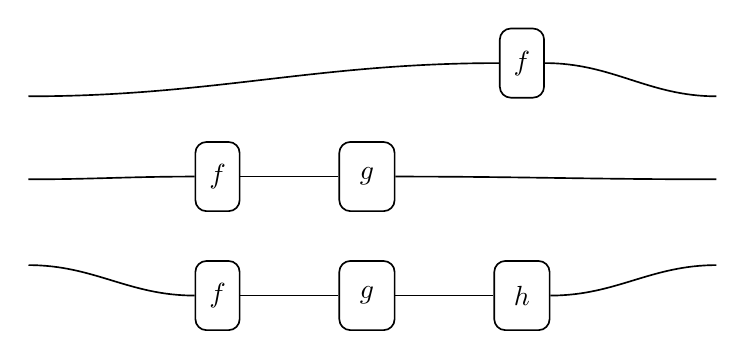
\begin{tikzpicture}[unit length/.code={{\newdimen\tikzunit}\setlength{\tikzunit}{#1}},unit length=1pt,x=\tikzunit,y=\tikzunit,semithick,box/.style={rectangle,draw,solid,rounded corners},outer box/.style={draw=none},wire/.style={draw}]
\node[outer box,minimum width=248\tikzunit,minimum height=109\tikzunit] (root) at (0,0) {};\node[box,minimum width=16\tikzunit,minimum height=25\tikzunit] (n3) at (54,42) {$f$};\node[box,minimum width=16\tikzunit,minimum height=25\tikzunit] (n4) at (-56,1) {$f$};\node[box,minimum width=20\tikzunit,minimum height=25\tikzunit] (n5) at (-2,1) {$g$};\node[box,minimum width=16\tikzunit,minimum height=25\tikzunit] (n6) at (-56,-42) {$f$};\node[box,minimum width=20\tikzunit,minimum height=25\tikzunit] (n7) at (-2,-42) {$g$};\node[box,minimum width=20\tikzunit,minimum height=25\tikzunit] (n8) at (54,-42) {$h$};\path[wire] ($(root.west)+(0,30)$) to[out=0,in=-180] (n3.west);\path[wire] (root.west) to[out=0,in=-180] (n4.west);\path[wire] ($(root.west)+(0,-31)$) to[out=0,in=-180] (n6.west);\path[wire] (n3.east) to[out=0,in=180] ($(root.east)+(0,30)$);\path[wire] (n4.east) to[out=0,in=-180] (n5.west);\path[wire] (n5.east) to[out=0,in=180] (root.east);\path[wire] (n6.east) to[out=0,in=-180] (n7.west);\path[wire] (n7.east) to[out=0,in=-180] (n8.west);\path[wire] (n8.east) to[out=0,in=180] ($(root.east)+(0,-31)$);
\end{tikzpicture}
\end{document}
